\documentclass{article}

% Language setting
% Replace `english' with e.g. `spanish' to change the document language
\usepackage[russian]{babel}

% Set page size and margins
% Replace `letterpaper' with `a4paper' for UK/EU standard size
\usepackage[a4rpaper,top=2cm,bottom=2cm,left=3cm,right=3cm,marginparwidth=1.75cm]{geometry}

% Useful packages
\usepackage{amsmath, amssymb, amsthm}
\usepackage{indentfirst}
\usepackage{graphicx, float}
\usepackage[colorlinks=true, allcolors=blue]{hyperref}
\setlength{\parskip}{5pt}
\setlength{\parindent}{20}
\title{Байесовы нейронные сети}
\author{Басов Дмитрий Константинович}
\date{}
\begin{document}
\maketitle

\section{Обозначения и сокращения}
$N(\mu, \sigma^2)$ — нормальное распределение

$\bold{x} \cdot \bold{y}$ — поэлементное произведение (произведение Адамара)

$\mathcal{L}$ — Evidence Lower Bound (ELBO)

$KL(q || p) = \int_{}{} q(\bold{Z}) \cdot \ln{\dfrac{q(\bold{Z})}{p(\bold{Z})}} d\bold{Z}$ — расстояние Кульбака — Лейблера

$\bold{x}$ — вектор признаков

$\bold{y}$ — таргет

$D$ — датасет — пары значений \{$\bold{x_i}$, $\bold{y_i}$\}, где $i = 1, \dots, L$

$\bold{W}$ — параметры модели — случайная величина размерности M

$p(D | \bold{W}) = \prod_{i=1}^{L} p(\bold{y_i} | \bold{x_i}, \bold{W})$ — правдоподобие (likelihood)

$p(\bold{W})$ — априорное распределение параметров модели (prior)

$p(\bold{W}| D)$ — апостериорное распределение параметров модели (posterior)

$p(D)$ — маргинальная вероятность датасета (evidence)

$q(\bold{W})$ — аппроксимация апостериорного распределения параметров модели

$p(\bold{W}, D) =
p(D | \bold{W}) \cdot p(\bold{W}) =
p(\bold{W}| D)\cdot p(D)$
— совместная вероятность параметров и данных

\section{Постановка задачи}
Постановка задачи следующая: у нас есть датасет $D$ и наша цель — смоделировать распределение $p(\bold{y} | \bold{x}, D)$. То есть мы хотим получить распределение вероятностей таргета $\bold{y}$ для неразмеченных $\bold{x}$, используя датасет D. Сделаем следующие преобразования:

$p(\bold{y} | \bold{x}, D) =
\int_{}{} p(\bold{y}, \bold{W} | \bold{x}, D) d\bold{W} =
\int_{}{} p(\bold{y} | \bold{W}, \bold{x}, D) \cdot p(\bold{W} | \bold{x}, D) d\bold{W} = 
\int_{}{} p(\bold{y} | \bold{W}, \bold{x}) \cdot p(\bold{W} | D) d\bold{W}$

Получим выражение для $p(\bold{W}| D)$, используя формулу Байеса:

$p(\bold{W}| D) =
\dfrac{p(\bold{W}, D)}{p(D)} =
\dfrac{p(\bold{W}, D)}{\int_{}{} p(\bold{W}, D) d\bold{W}} =
\dfrac{p(D | \bold{W}) \cdot p(\bold{W})}{\int_{}{} p(D | \bold{W}) \cdot p(\bold{W}) d\bold{W}} $

Для аппроксимации распределения ответов модели можно воспользоваться методом Монте — Карло: взять сэмпл весов $\hat{\bold{W}}$ из $p(\bold{W}| D)$, прогнать их через модель и получить $\hat{\bold{y}}$. Однако для этого необходимо уметь сэмплировать из распределения $p(\bold{W}| D)$.

Получить аналитическое решение можно только в очень ограниченном числе случаев. Существует возможность сэмплировать из $p(\bold{W}| D)$, используя методы Монте — Карло для марковских цепей (MCMC). Однако для больших датасетов и большого числа параметров это становится технически сложно. Альтернативный подход к решению таких задач — аппроксимация распределения $p(\bold{W}| D)$ распределением $q(\bold{W})$, из которого сэмплировать намного проще.


\section{Вариационный вывод для нейронной сети}
Запишем выражение ELBO для распределения $q(\bold{W})$ и преобразуем его, используя тождество $p(\bold{W}, D) = p(\bold{W}| D)\cdot p(D)$:

$
\mathcal{L}(q(\bold{W})) =
\int_{}{} q(\bold{W}) \cdot \ln{\dfrac{p(\bold{D}, \bold{W})}{q(\bold{W})}} d\bold{W} =
\int_{}{} q(\bold{W}) \cdot \ln{\dfrac{p(\bold{W}| D) \cdot p(D)}{q(\bold{W})}} d\bold{W} = 
\ln{p(D)} \cdot \int_{}{} q(\bold{W}) d\bold{W} - \int_{}{} q(\bold{W})\cdot \ln{\dfrac{q(\bold{W})}{p(\bold{W}| D)}} d\bold{W} =
\ln{p(D)} - KL(q(\bold{W}) || p(\bold{W}| D))
$

Из равенства $\mathcal{L}(q(\bold{W})) = ln(p(D)) - KL(q(\bold{W}) || p(\bold{W}| D))$ видно, что максимизируя $\mathcal{L}(q(\bold{W}))$, мы не только максимизируем $\ln {p(D)}$, но и минимизируем $KL(q(\bold{W}) || p(\bold{W}| D))$. То есть распределение $q(\bold{W})$ будет приближаться к распределению $p(\bold{W}| D)$.

Будем максимизировать $\mathcal{L}(q(\bold{W}))$. Преобразуем выражение для $\mathcal{L}(q(\bold{W}))$, используя тождество
$p(\bold{W}, D) = p(D | \bold{W}) \cdot p(\bold{W})$:

$
\mathcal{L}(q(\bold{W})) =
\int_{}{} q(\bold{W}) \cdot \ln{\dfrac{p(\bold{D}, \bold{W})}{q(\bold{W})}} d\bold{W} =
\int_{}{} q(\bold{W}) \cdot \ln{\dfrac{p(D | \bold{W}) \cdot p(\bold{W})}{q(\bold{W})}} d\bold{W} = 
\int_{}{} q(\bold{W}) \cdot \ln{p(D | \bold{W})} d\bold{W} - \int_{}{} q(\bold{W}) \cdot \ln{\dfrac{q(\bold{W})}{p(\bold{W})}} = 
\int_{}{} q(\bold{W}) \cdot \ln{p(D | \bold{W})} d\bold{W} - KL(q(\bold{W}) || p(\bold{W}))
$

Для дальнейшнего вывода положим, что распределения $p(\bold{W})$ и $q(\bold{W})$ являются нормальными с диагональными матрицами ковариации:

$p(\bold{W}) = N(\bold{W} | \bold{0}, \pmb{\sigma_{p(\bold{W})}}^{2} \cdot \bold{I})$, где $\pmb{\sigma_{p(\bold{W})}}$ — вектор длины M

$q(\bold{W}) = N(\bold{W} | \pmb{\mu}, \pmb{\sigma_{q(\bold{W})}}^{2} \cdot \bold{I})$, где $\pmb{\mu}$ и $\pmb{\sigma_{q(\bold{W})}}$ — вектора длины M

Так как распределения $p(\bold{W})$ и $q(\bold{W})$ являются нормальными, то $KL(q(\bold{W}) || p(\bold{W}))$ можно посчитать аналитически:

$
KL(q(\bold{W}) || p(\bold{W})) = 
\dfrac{1}{2}\sum_{k=1}^{M}(\dfrac{\sigma_{{q(W)_{k}}}^2}{\sigma_{{p(W)_{k}}}^2} + \dfrac{\mu_{k}^2}{\sigma_{{p(W)_{k}}}^2} - \ln{\dfrac{\sigma_{{q(W)_{k}}}^2}{\sigma_{{p(W)_{k}}}^2}} - 1)
$

Априорное распределение параметров модели определяется параметром $\pmb{\sigma_{p(\bold{W})}}$. Воспользуемся техникой эмпирического Байеса — нахождения параметров априорного распределения из данных. Посчитаем
$\dfrac{d\mathcal{L}(q(\bold{W}))}{d ({\sigma_{p(W)_{k}}^{-2}})}$:

$
\dfrac{d\mathcal{L}(q(\bold{W}))}{d ({\sigma_{p(W)_{k}}^{-2}})} =
\dfrac{d (\int_{}{} q(\bold{W}) \cdot \ln{p(D | \bold{W})} d\bold{W} - KL(q(\bold{W}) || p(\bold{W})))}{d ({\sigma_{p(W)_{k}}^{-2}})} =
- \dfrac{d (KL(q(\bold{W}) || p(\bold{W})))}{d ({\sigma_{p(W)_{k}}^{-2}})}$

$
\dfrac{d\mathcal{L}(q(\bold{W}))}{d ({\sigma_{p(W)_{k}}^{-2}})} =
-\dfrac{1}{2}\sum_{k=1}^{M}(\sigma_{{q(W)_{k}}}^2 + \mu_{k}^2 - \sigma_{{p(W)_{k}}}^2)
$

Приравняв производную к нулю, получим:

$
-\dfrac{1}{2}\sum_{k=1}^{M}(\sigma_{{q(W)_{k}}}^2 + \mu_{k}^2 - \sigma_{{p(W)_{k}}}^2) = 0
$

$
(\sigma_{{q(W)_{k}}}^2 + \mu_{k}^2 - \sigma_{{p(W)_{k}}}^2) = 0
$

$\pmb{\sigma_{p(\bold{W})}^{2}} = \pmb{\mu^{2}} + \pmb{\sigma_{q(\bold{W})}^{2}}$

Подставив полученное выражение в $KL(q(\bold{W}) || p(\bold{W}))$, получим:

$
KL(q(\bold{W}) || p(\bold{W})) = 
\dfrac{1}{2}\sum_{k=1}^{M}\ln({1 + \dfrac{\mu_{k}^2}{\sigma_{{q(W)_{k}}}^2}})
$

Чтобы избежать неопределенности $\dfrac{0}{0}$, и чтобы $\pmb{\sigma_{q(\bold{W})}}$ была всегда положительна, сделаем следующую замену переменных:

$\mu_{k} = \gamma_{k} \cdot e^{\rho_{k}}$

$\sigma_{{q(W)_{k}}} = |\gamma_{k}|$

Тогда: 

$
KL(q(\bold{W}) || p(\bold{W})) = 
\dfrac{1}{2}\sum_{k=1}^{M}\ln({1 + \dfrac{\mu_{k}^2}{\sigma_{{q(W)_{k}}}^2}}) = 
\dfrac{1}{2}\sum_{k=1}^{M}\ln({1 + e^{2 \cdot \rho_{k}}}) = 
\dfrac{1}{2}\sum_{k=1}^{M}Softplus(2 \cdot \rho_{k})
$

Таким образом, функция потерь будет иметь следующий вид:

$
Loss(\pmb{\rho}, \pmb{\gamma}) =
- \dfrac{\mathcal{L}(q(\bold{W}))}{L} =
\int_{}{} N(\bold{W} | \pmb{\mu}, \pmb{\sigma_{q(\bold{W})}}^{2} \cdot \bold{I}) \cdot NLL \cdot d\bold{W} + \dfrac{KL}{L}
$, где:

$\pmb{\mu} = \pmb{\gamma} \cdot \exp({\pmb{\rho}})$

$\pmb{\sigma_{q(\bold{W})}} = |\pmb{\gamma}|$

$NLL = -\dfrac{1}{L}\sum_{i=1}^{L}{\ln{p( \bold{y_{i}} | \bold{x_{i}}, \bold{W})}}$

$KL = \dfrac{1}{2}\sum_{k=1}^{M}Softplus(2 \cdot \rho_{k})$

\section{Алгоритм обучения}
Задаем шаг градиентного спуска $\alpha$ и инициализируем параметры распределения $q(\bold{W})$ — $\pmb{\rho}$ и $\pmb{\gamma}$. Затем повторяем, пока не достигнем критерия остановки:
\begin{enumerate}
    \item $\pmb{\sigma} \leftarrow |\pmb{\gamma}|$
    \item $\pmb{\mu} \leftarrow \pmb{\gamma} \cdot \exp({\pmb{\rho}})$
    \item $\hat{\bold{W}} \leftarrow N(0, 1)$ — сэмплируем случайные веса
    \item $\hat{\bold{W}} \leftarrow \hat{\bold{W}} \cdot \pmb{\sigma} + \pmb{\mu}$ — репараметризация
    \item $nll \leftarrow -\dfrac{1}{L}\sum_{i=1}^{L}{\ln{p( \bold{y_{i}} | \bold{x_{i}}, \bold{\hat{W}})}}$
    \item $kl \leftarrow \dfrac{1}{2}\sum_{k=1}^{M}Softplus(2 \cdot \rho_{k})$
    \item $l \leftarrow nll + \dfrac{kl}{L}$ — считаем функцию потерь
    \item $\pmb{\rho} \leftarrow \pmb{\rho} - \alpha \dfrac{d l}{d \pmb{\rho}}$
    \item $\pmb{\gamma} \leftarrow \pmb{\gamma} - \alpha \dfrac{d l}{d \pmb{\gamma}}$
\end{enumerate}

\section{Эксперименты}

Для проверки своей гипотезы я выбрал \href{https://www.kaggle.com/datasets/rabieelkharoua/alzheimers-disease-dataset}{Alzheimer's Disease Dataset}. Данные были разбиты на тренировочную и тестовую часть в пропорции 80 на 20. В качестве архитектуры была выбрана полносвязная нейронная сеть с одним скрытым слоем и функцией активации ReLU. То есть:

$z = ReLU(matmul(x, W_1))$

$y = Sigmoid(matmul(z, W_2))$

Размерность скрытого состояния $z$ варьировалась от 1 до 37. Для каждой размерности обучались 2 модели - классическая (без регуляризации) и байесовская. Для каждой модели производилась оценка ROC-AUC на тренировочной и тестовой выборках. На рисунках 1 и 2 представлены результаты экспериментов

\begin{figure}
    \centering
    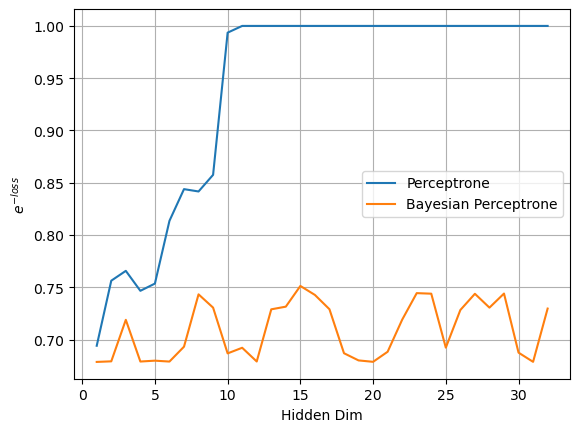
\includegraphics[width=1\linewidth]{loss.png}
    \caption{Зависимость $e^{-loss}$ от размерности скрытого состояния на тренировочных данных}
    \label{fig:enter-label}
\end{figure}

\begin{figure}
    \centering
    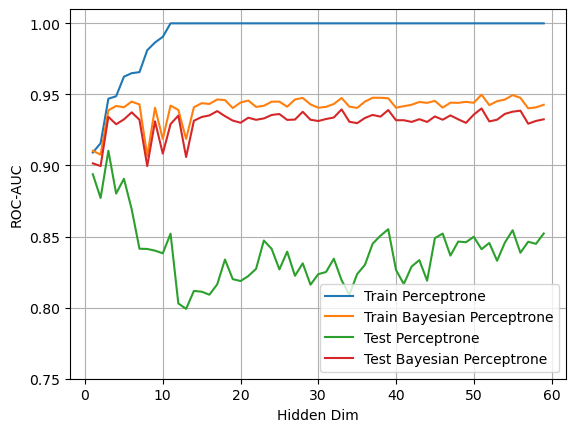
\includegraphics[width=1\linewidth]{roc_auc.png}
    \caption{Зависимость $ROC-AUC$ от размерности скрытого состояния на тренировочных и тестовых данных}
    \label{fig:enter-label}
\end{figure}

\section{Выводы}
По результатам работы можно сделать следующие выводы:
\begin{itemize}
    \item с ростом сложности модели байесова нейронная сеть не переобучилась;
    \item качество на тестовой выборке на всём рассматриваемом диапазоне гиперпараметров у байесовой нейронной сети было выше, чем у классической;
    \item значение ROC-AUC на тестовой выборке имеет очень высокую корреляцию со значением ROC-AUC на тренировочной выборке (0.97 по Пирсону). Следовательно, для подбора гиперпараметров можно ориентироваться на метрики, полученные по тренировочной выборке. Это даёт нам возможность отказаться от деления на тренировочную и валидационную выборки для подбора гиперпараметров.
\end{itemize}

Так же стоит отметить, что данный подход переносится на другие архитектуры нейронных сетей (рекуррентные, свёрточные, трансформеры).

Имплементация данного подхода была выполнена с использованием PyTorch. Весь исходный код для проведения экспериментов размещён по адресу \url{https://github.com/dimabasow/bayesian-neural-networks}.

\end{document}
